% !TeX root = ../../main.tex
\section{Introduction}


\section{Choice of separator}
The separation of p-nitrotoluene from m-nitrotoluene was designed in detail. P-nitrotoluene is an essential precursor to aminobenzaldehyde and aminobenzoic acid therefore it needs to be purified to at least --- \%. Due to the small difference in boiling points between p-NT and m-NT, distillation is infeasible and energy intensive. Similar solubility between the two components made the use of absorption or adsorption processes infeasible as well. However, crystallisers are deemed feasible due to the difference in melting points between p-nitrotoluene and m-nitrotoluene.

*Table of boiling points, melting points and mole fraction 

Melt crystallisers are particularly good for separating organic chemicals with favourable melting points. Compared to solution crystallisers, the concentration of the key component is usually much higher, and the growth rate in melt crystalliser is relatively fast. This leads to high purity of products and is thus economically favourable. It also avoids the possibility  of thermal degradation because it is typically operated at a cool temperature (1). From an environmental perspective, solution crystallisation often involves the addition of a solvent that is usually treated as impurity, whereas melt crystallisation does not require any additional substance. Melt crystalliser also known to be relatively cheaper - need to find cost info if possible.

Types of melt crystallisers include primarily solid-layer and suspension. 
Solid layer crystalliser:
advantages: avoid encrustation issue
disadvantages: higher investment costs, multistage process, not commonly used as continuous process

Suspension crystalliser:
advantages: moderate crystal growth and large surface areas, high purity product, continuous operation mode.
disadvantages: slurry handling,extras washing step required for solid-liquid separation, moving parts (1). 

Since the plant aims to operate continuously suspension crystalliser was more suitable than solid-layer crystalliser. A novel crystalliser known as mixed-suspension mixed-product removal (MSMPR) was chosen. It operates continuously by producing a slurry of p-nitrotoluene crystals and m-nitrotoluene liquid which will be further separated in a hydraulic wash column to attain purified molten p-nitrotoluene. 

Jaksland analysis?

Alternatives considered..

*Table of comparison between type of crystallisers

 




\section{Crystalliser design}
\subsection{(p-Nitrotoluene + m-nitrotoluene) phase behaviour}

The (p-nitrotoluene + m-nitrotoluene) system exhibits a eutectic-forming solid-liquid phase behaviour. In such a system, one of the two components is able to crystallise out from the homogeneous liquid as pure solid when cooled below the binary melting point. 

\subsection{Population balance of MSMPR crystallisation}
In order to specify a MSMPR crystallisation process, it is important to determine the crystal population balance. The population balance, together with the mass balance, accounts for the crystal size distribution (CSD) where information about the kinetics of crystal formation is contained. The population balance has been a central focus in the works of Randoph and Larson. 

First, for many commercial crystallisation processes, McCabe's $\Delta$ L law is generally applied, 

\begin{equation} \label{eq: McCabe deltaL}
    \Delta L = G \Delta t
\end{equation}

\noindent where $L$ is the characteristic size of crystal, $t$ is time, and $G$ is the growth rate whose dimensions are length per unit time. The main assumption is that the crystal growth rate is independent of crystal size. 

Then, the crystal population density, $n$, defined as the number of crystals per unit size per unit volume, is expressed as 

\begin{equation} \label{eq:crystal population density definition}
    .
\end{equation}


\subsection{Heat transfer}





























\section{Hydraulic wash column design}

Commonly used solid-liquid separators are not continuous processes, typically batch or semi-batch. Wash column does wash and continuous transport in one process. Whereas, for example a centrifuge would require  melting the crystals and a means of solid transport by conveyor belt. Different type of wash columns include gravity, hydraulic and mechanical. Hydraulic was chosen because of shorter residence time and less moving mechanical parts. 

\subsection{Steady State Model}  \textcolor{red}{We could put this in Appendix it's just repeating equations from literature.} 

Typically, the design of a hydraulic wash column will be based on pilot-scale experiments to determine appropriate dimensions at varying operating conditions. Instead, a  model from literature --- was used to estimate the performance of the column at steady state. The hydraulic wash column was modelled based on volume and force balance using initial dimensions from ---. The initial dimensions were varied to determine the performance of the column for output from the MSMPR crystalliser. 

The model assumes 100 \% solid-liquid separation in the wash column therefore no presence of liquid in the product flow rate because the pressure difference is large enough to ensure no mother liquor enters the wash front. However, if impurities are entrapped in the crystal lattice during crystallisation, these will not be removed. This highlights the disadvantage of hydraulic wash column compared to gravity wash column. Gravity wash column allows some impurities to be removed from the crystals during the long residence time. 

** a diagram of the wash column

\textbf{Volume balance} 
This model was based on the assumption that the liquid and solid in the system were incompressible. For simplicity density and viscosity were assumed to be independent of temperature. 

Overall volume balance at the top section 
\begin{equation}
\phi_{feed}+\phi_{steer}=\phi_{s,filters}+\phi_{ml.filters}
\end{equation}

The total length of the top section is constant. The length of the filtration section was derived from the solid balance in the top section. 

\begin{equation}
\frac{dL_{filtration}}{dt} = \frac{1}{A_c(1-\alpha_2-\epsilon)}(\alpha_1\phi_{feed}-\phi_{s,filters})
\end{equation}

In the bottom section, there is the stagnant zone with the crystals. Then there is the wash zone with only the crystal and the wash liquid at steady state. The wash liquid crystallises due to the low temperature at the wash front. The crystallisation of the wash liquid can be related to the disappearance of the wash liquid by difference in density of the solid and liquid.

\begin{equation}
C_l= \frac{\rho_s}{\rho_l}C_s
\end{equation}

The amount of crystallised material was calculated based on a heat balance and temperature difference between the feed and the melt. This assumes the total cooling capacity of the crystals is used to crystallise the wash liquid. 

\begin{equation}
C_s= \frac{c_p(T_{melt}-T_{feed})}{\Delta H_m}Q_{s,filters}
\end{equation}

The length of the wash section is related to the wash-liquid flow entering the knife and the wash liquid that crystallises. This assumes the wash liquid is not loss through the filters which is ensured by positioning the filters above the wash section.

\begin{equation}
\epsilon_w A_c \frac{dL_{wash}}{dt}= \phi_{wl,knife}-C_l
\end{equation}

The wash column during operation forms 3 layers of filtration, stagnant and wash sections. Within the filtration and stagnant section it is assumed the porosity and permeability remain constant. Since the crystals form a densely packed column $\epsilon$ was taken as 0.45. Due to the wash-liquid crystallisation at the wash zone an abrupt change in porosity and permeability was considered. The consolidation of the crystal bed were neglected in this model, however under compressive force from the pressure at the top section this may not be a valid assumption and will have to be further evaluated in a pilot scale experiment. The porosity in the wash zone was calculated from the equation below. 

\begin{equation}
\epsilon_{w}= \epsilon-(1-\epsilon)\left(\frac{c_p(T_{melt}-T_{feed})}{\Delta H_m}\right)
\end{equation}

At steady state, the wash section is constant therefore there  would be no flow of mother liquor into or out of the bottom section. The mother liquor at the top section leaves the column through the filter and splits into residual and steer flow. 

\begin{equation}
\phi_{residue}= \phi_{ml,filters} - \phi_{steer}
\end{equation}

The volume balance at the melting circuit is based on the assumption that crystals are molten the moment they enter the melting circuit. The wash liquid enters the column at the melting temperature. 

\begin{equation}
\frac{\rho_s}{\rho_l}\phi_{s,knife}= \phi_{wl,knife} - \phi_{product}
\end{equation}


\textbf{Force balance}
\\The liquid pressure drop across each section were calculated with the following modified Darcy's law equation. 

\begin{equation}
\frac{\Delta P_{l,filtration}}{L_{filtration}}=\frac{\epsilon \eta_{l}}{B_{filtration}}\left(\frac{\phi_{ml,filters}}{\epsilon A_c} - \frac{\phi_{s,filters}}{1-\epsilon A_c}\right)
\end{equation}

\begin{equation}
\frac{\Delta P_{l,stagnant}}{L_{stagnant}}=\frac{\epsilon \eta_{l}}{B_{stagnant}}\left(-\frac{\phi_{ml,bottom}}{\epsilon A_c} - \frac{\phi_{s,filters}}{1-\epsilon A_c}\right)
\end{equation}

\begin{equation}
\frac{\Delta P_{l,wash}}{L_{wash}}=\frac{\epsilon \eta_{l}}{B_{wash}}\left(-\frac{\phi_{wl,knife}}{\epsilon_w A_c} - \frac{\phi_{s,knife}}{1-\epsilon_w A_c}\right)
\end{equation}

The liquid pressure gradient at each section were assumed to be constant due to the incompressibilty assumption of the packed bed. The liquid pressure at the top in the slurry section was based on the pressure at the filter and the pressure drop over the filtration section. 

\begin{equation}
P_{top} = P_{filters} + \Delta P_{l,filtration}
\end{equation}


The pressure at the bottom is equal to the pressure drop in the valve of the melting circuit. This pressure drop across the valve is determined through a linear relation with the product flow rate.

\begin{equation}
P_{bottom}=\Delta P_{valve} = K_w\phi_{product}
\end{equation}

%The pressure after the valve is atmospheric.
The pressure in the melting circuit was calculated using the equation below. 

\begin{equation}
\Delta P_{valve} = \Delta P_{l,stagnant} + \Delta P_{l,wash} + P_{filters}
\end{equation}


\subsection{Results and Discussion}
The linear system of equations from the steady state model were solved using input variables and parameters shown in Table --. 

\begin{table}[h]
\centering
\caption{Input variables and parameters}
\label{tab:inputsparameters}
\begin{tabular}{lll|lll}
\multicolumn{3}{c|}{Inputs}          & \multicolumn{3}{c}{Parameters}             \\ \toprule
$\phi_{feed}$  & $4.27\times10^{5}$ & m^{3}/s &
$\epsilon$  & 0.45  & - \\ \hline
$\phi_{steer}$    & $1.8\times10^{5}$ & m^{3}/s &
B_{filtration}  & $7.87\times10^{-14}$ & m^{2} \\ \hline
$\alpha_1$ & 0.801  & v/v &
B_{wash}  & $6.75\times10^{-14}$ & m^{2} \\ \hline
K_{w} &  $2.8\times10^{10}$ & Pas/m^{3}  & &  &  \\ \bottomrule
\end{tabular}
\end{table}


Final dimension table - Length of bed, height, diameter, number of filter tubes etc. 

During operation of the hydraulic column  variations in the length of the filtration, stagnant and wash section with time was expected. Therefore, simulations of variable filtration and wash section lengths were implemented on Excel to determine the effect on pressures at different points in the column. With proper controls in place, the sections should not vary significantly during normal operation, therefore the range for variation in filtration and wash section were taken between 0.28 to 0.30 m.  

\begin{figure}[h]
  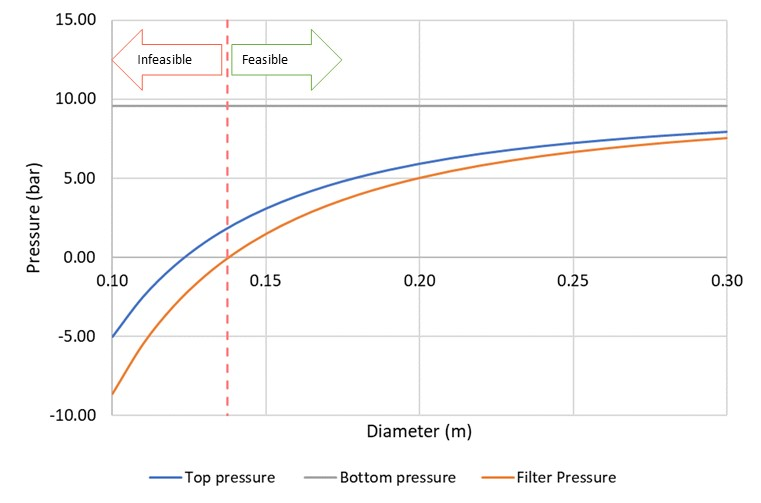
\includegraphics[scale=0.5]{chapters/3-separation/figures/diameter.jpg}
  \caption{Effect of varying diameter.}
  \label{fig:dia_col}
\end{figure}


*graph on effect of varying diameter 
\\In the design of the hydraulic column there are many variables included. Therefore, the length of the variable was fixed at 1 m following the literature. Instead, the diameter of the column was varied. Figure -- shows the impact diameter has on the column's performance. Below 0.165 m the model showed negative pressure at the filter implying instead of mother liquor flowing up through the filter tube, it could be flowing in the reverse direction. The pressure at the top is also negative indicating at these conditions the fluid flow in the column may not be in the desirable downward direction. A suitable diameter was chosen at 0.17 m allowing for slight variations in the section lengths over time under normal operation. 

\begin{figure}[h]
  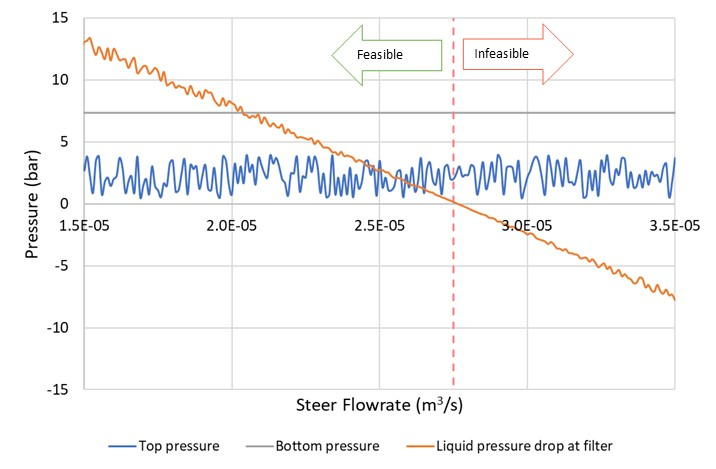
\includegraphics[scale=0.5]{chapters/3-separation/figures/steerflow.jpg}
  \caption{Effect of varying steer flowrate}
  \label{fig:steer_col}
\end{figure}

*graph on effect of varying steer flow 
\\Steer flow is the flow rate of the mother liquor being recycled back into the column from the filter tubes whilst some mother liquor are removed as residual flow. In order to find the appropriate steer flow, it was varied from 4.5e-6 to 3.45e-5 m3/s. Figure -- shows the unfeasible and feasible region of operation. Above a steer flow 2e-5, the column starts exhibiting negative liquid pressure drop at the filter. However, at lower steer flow such as 4.5e-6 the filter pressure increases significantly to more than 15 bar. In order to attain a lower pressure but also ensure the column is in a feasible region, the steer flow at 1.8 e-5 was chosen as reasonable. At this flow rate there is an allowance for variation in the flowrate whilst the column is still operating in the feasible region. 

\begin{figure}[h]
  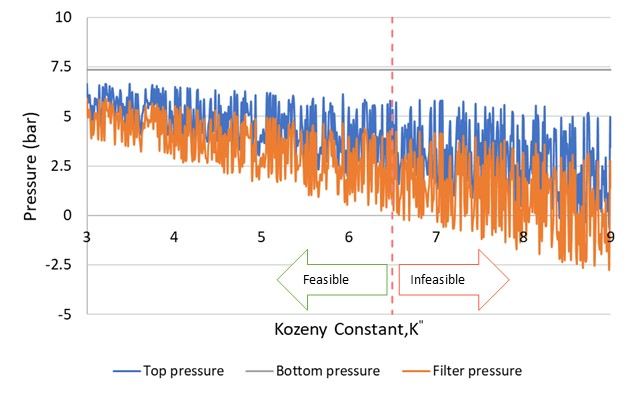
\includegraphics[scale=0.5]{chapters/3-separation/figures/kozeny.jpg}
  \caption{Effect of varying Kozeny constant}
  \label{fig:koz_col}
\end{figure}
*graph on effect of varying permeability constant

\\A sensitivity analysis on the permeability constant was conducted by varying the Kozeny constant, K. 


\subsection{Materials Choice}
- material for the column itself 

\subsection{Mechanical Design}
-BS5500 standard has to be followed since column maximum operating pressure is 9.8 bar. It is a pressure vessel.  
